% !TEX root = ./main.tex

\documentclass{article}
\usepackage[utf8]{inputenc}
\usepackage{pdfpages}
\usepackage{graphicx}
\graphicspath{ {./img/} }

\usepackage{listings}
\usepackage{xcolor}

\definecolor{codegreen}{rgb}{0,0.6,0}
\definecolor{codegray}{rgb}{0.5,0.5,0.5}
\definecolor{codepurple}{rgb}{0.58,0,0.82}
\definecolor{backcolour}{rgb}{0.95,0.95,0.92}

\lstdefinestyle{mystyle}{
    backgroundcolor=\color{backcolour},   
    commentstyle=\color{codegreen},
    keywordstyle=\color{magenta},
    numberstyle=\tiny\color{codegray},
    stringstyle=\color{codepurple},
    basicstyle=\ttfamily\footnotesize,
    breakatwhitespace=false,         
    breaklines=true,                 
    captionpos=b,                    
    keepspaces=true,                 
    numbers=left,                    
    numbersep=5pt,                  
    showspaces=false,                
    showstringspaces=false,
    showtabs=false,                  
    tabsize=2
}

\lstset{style=mystyle}
\lstset{literate=%
{Ö}{{\"O}}1
{Ä}{{\"A}}1
{Ü}{{\"U}}1
{ß}{{\ss}}2
{ü}{{\"u}}1
{ä}{{\"a}}1
{ö}{{\"o}}1
}


\title{Aktorik Sensorik \\ Labor 1}
\author{Anton Kress (S872899), Jan Abel (S876662)}
\date{October 2020}

\begin{document}

\maketitle


\section*{Aufgabenstellung}

\begin{figure}[htp]
 \centering
 \includegraphics[page=3, width=0.8\textwidth]{Aufgabenstellung.pdf}
 %\caption{Aufbau der CBM-Toolchain}
 \label{fig:Aufgabenstellung A1}
\end{figure}


\section{Messung des Stillstandsdrehmomentes}

\subsection{Beschreibung}

Im ersten Versuch soll die Momentenkonstante $k_m$ bestimmt werden.
Sie hängt folgendermaßen mit dem Drehmoment $M_M$ und dem Motorstrom $i_a(t)$
zusammen. 

\begin{equation} \label{eq111}
    \begin{split}
        M_M(t)&=k_m \cdot i_a(t)\\
        k_m&=\frac{M_M(t)}{i_a(t)}
    \end{split}
\end{equation}

Als Messwerte ist eine Matrix mit den Motorströmen $I_a$ und der Auslenkungskraft $F$
gegeben. Um daraus das Drehmoment $M_M$ zu bestimmen wird der Radius $r$ benötigt,
welcher mit $1 \mathrm{cm}$ gegeben ist.

\begin{equation} \label{eq112}
    \begin{split}
        M_M=f(I_a)&=r \cdot F(I_a)
    \end{split}
\end{equation}

Anschließend kann die Momentenkonstante $k_m$ über die Steigung der geplotteten
Gerade bestimmt werden. Hierfür muss gewährleistet werden, dass der Arbeistpunkt
linear ist. Deshalb dürfen die letzten drei Messwerte in der linearen Regression
nicht betrachtet werden.

\begin{equation} \label{eq113}
    \begin{split}
        k_m\simeq 0.022 \mathrm{\frac{Nm}{A}}
    \end{split}
\end{equation}


% \lipsum[1]\\




\subsection{Ausgabe der Lösung}
\begin{figure}[H]
 \centering
 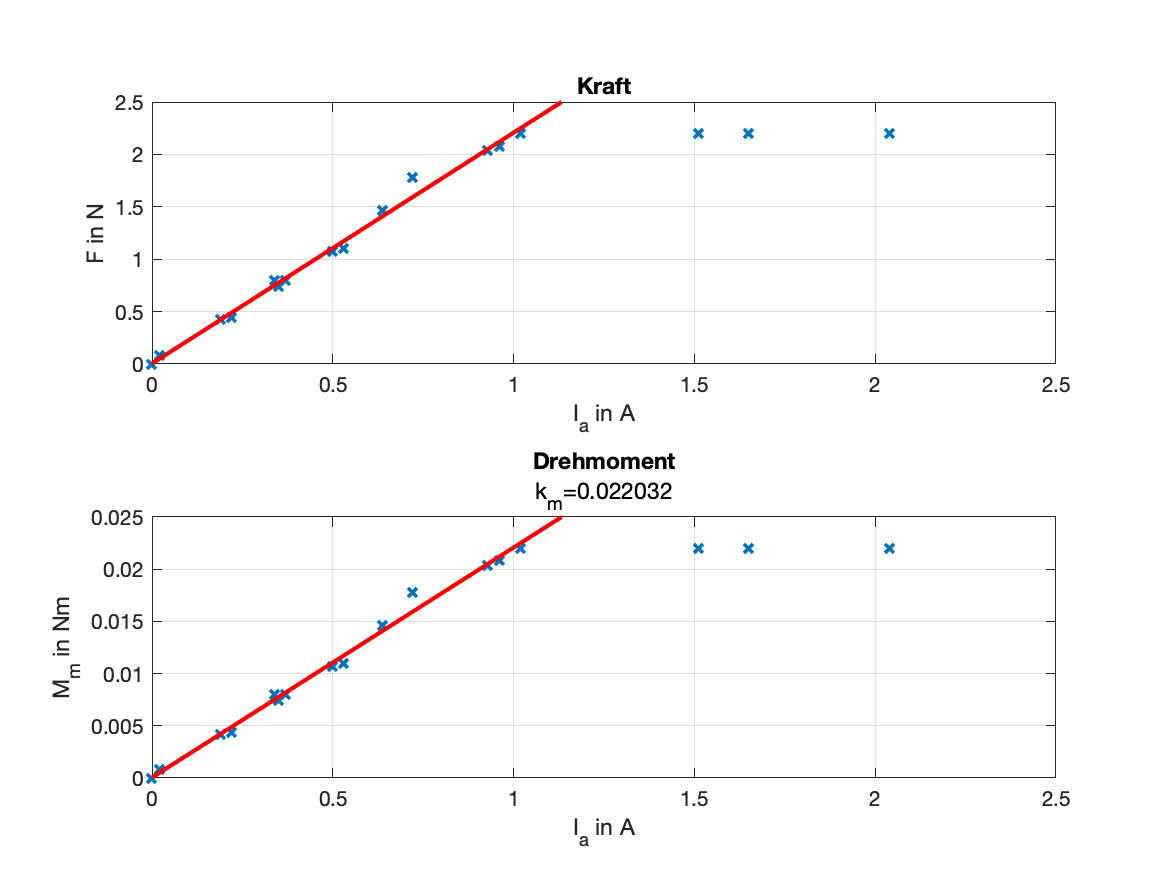
\includegraphics[width=1\textwidth]{as_labor01_1.png}
 \caption{Plot der Aufgabe 1}
 \label{fig:PlotAufgabe1}
\end{figure}

\subsection{Matlab Code}
\lstinputlisting[language=Matlab]{matlab/as_labor01_1.m}

\section{Messung des Ankerwiderstand}

\subsection{Beschreibung}

Im zweiten Versuch soll der Ankerwiderstand $R$ bestimmt werden.
Der Ankerwiderstand kann über das Ohm'sche Gesetz berechnet werden,
dafür ist eine Matrix mit den Messwerten der Spannungen und Ströme gegeben.
Da mit den Messwerten die Ströme über den Spannungen abgebildet werden ist die
Steigung nicht der Widerstand sondern der Leitwert. Deshalb muss zur Ermittlung
des Ankerwiderstand noch das Reziproke des Leitwerts berechnet werden.

\begin{equation} \label{eq121}
    \begin{split}
        R&=\frac{U_a}{I_a} \Leftrightarrow G=\frac{1}{R}=\frac{I_a}{U_a}\\
        R&\simeq 3.26 \mathrm{\Omega}
    \end{split}
\end{equation}

\subsection{Ausgabe der Lösung}
\begin{figure}[H]
 \centering
 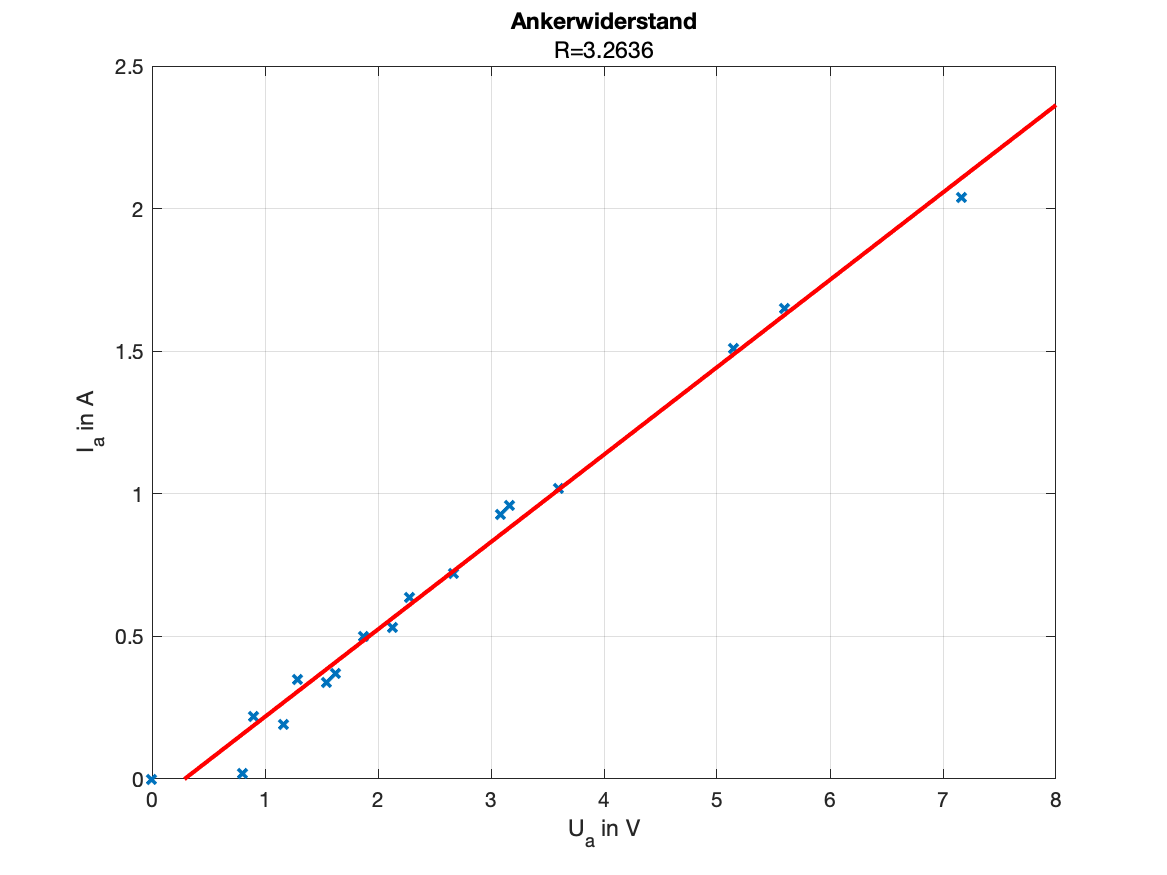
\includegraphics[width=1\textwidth]{as_labor01_2.png}
 \caption{Plot der Aufgabe 2}
 \label{fig:PlotAufgabe2}
\end{figure}

\subsection{Matlab Code}
\lstinputlisting[language=Matlab]{matlab/as_labor01_2.m}

\section{Messung des Stillstandsdrehmomentes}

\subsection{Beschreibung}
\lipsum[1]\\

\subsection{Ausgabe der Lösung}
\begin{figure}[htp]
 \centering
 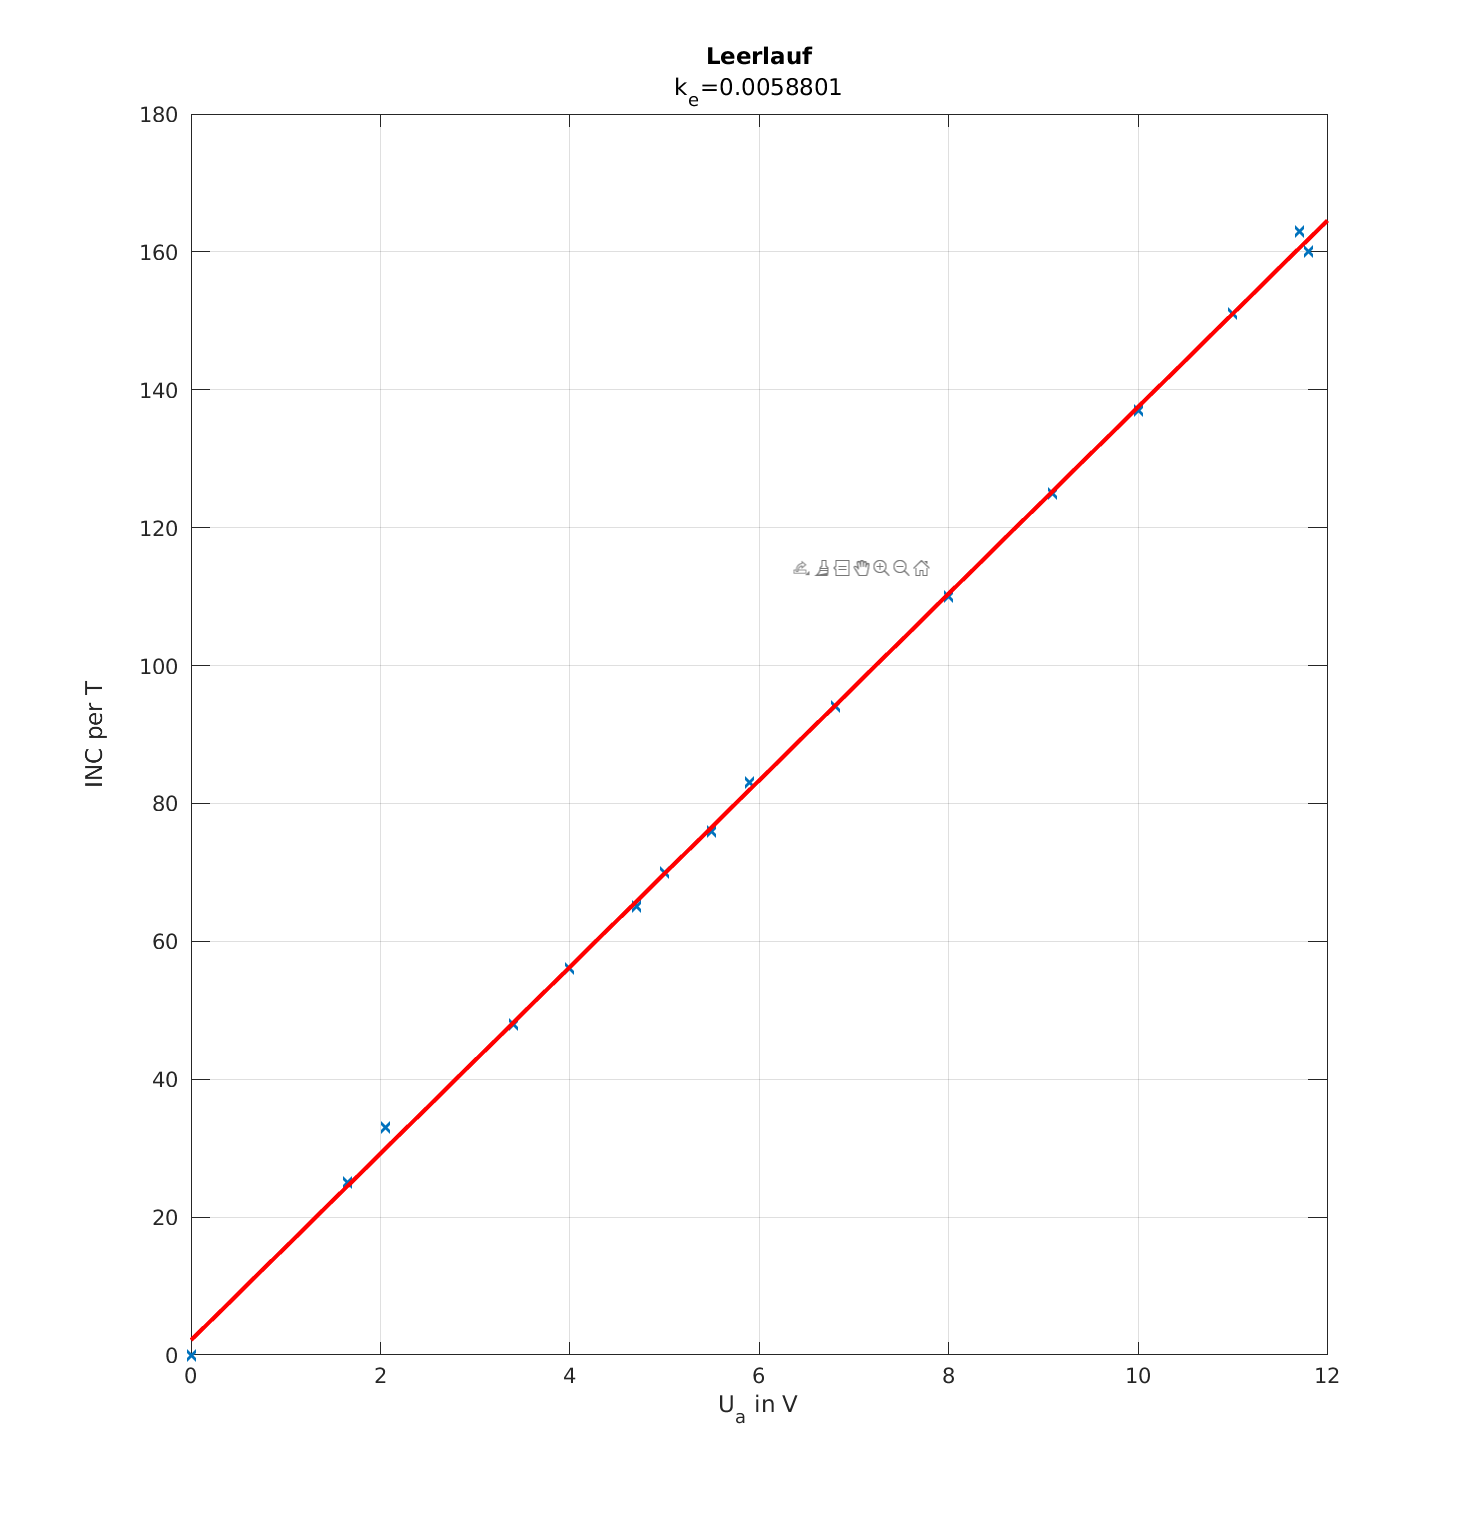
\includegraphics[width=1\textwidth]{as_labor01_3.png}
 \caption{Plot der Aufgabe 3}
 \label{fig:PlotAufgabe3}
\end{figure}

\subsection{Matlab Code}
\lstinputlisting[language=Matlab]{matlab/as_labor01_3.m}

\section{Messung der Kennlinie des Verstärkers}

\subsection{Beschreibung}

In der letzten Messung soll die Kennlinie des Messverstärkers ermittelt
werden und damit der Verstärkungsfaktor $A$ bestimmt werden. Dafür liegt
eine Matrix mit den Eingangsspannungen $U_e$ und den Ausgangspannungen
$U_a$ vor.
Da der Verstärker Ausgangsseitig bei etwa $+13.75\mathrm{V}$ und 
$-13.06\mathrm{V}$ in Sättigung geht, werden die jeweils ersten 2
und die letzten beide Werte nicht betrachtet.

Die Steigung der linearen Funktion ist 

Der Verstärkungsfaktor $A$ ist der Quotient aus Ausgangs- und Eingangsspannung
und somit die Steigung.

\begin{equation} \label{eq141}
    \begin{split}
        A=\frac{U_a}{U_e}\simeq2 \mathrm{V}
    \end{split}
\end{equation}



\subsection{Ausgabe der Lösung}
\begin{figure}[H]
 \centering
 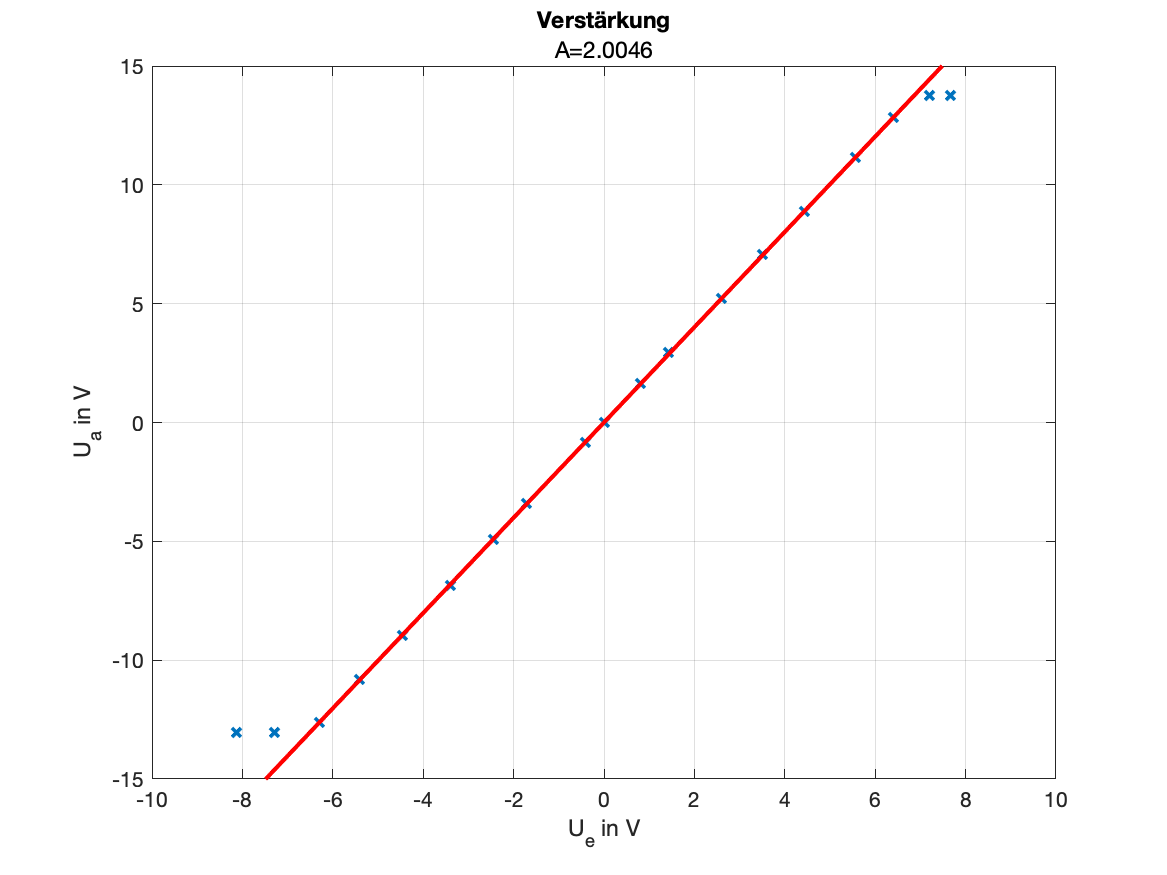
\includegraphics[width=1\textwidth]{as_labor01_4.png}
 \caption{Plot der Aufgabe 4}
 \label{fig:PlotAufgabe4}
\end{figure}

\subsection{Matlab Code}
\lstinputlisting[language=Matlab]{matlab/as_labor01_4.m}


\end{document}
